

\section{Background}

The statement of site percolation is quite simple: every site in a lattice is either occupied with a probability $p$ or not with probability $1-p$. Neighboring occupied sites are grouped into clusters. At a specific value of $p$, we can observe an interesting phenomenon: the formation of a cluster spanning the entire system. This is called percolation. In the limit of an infinite lattice, there is a finite threshold probability $p_c$ such that~\cite{Gould_2006}:
\begin{itemize}
	\item for $p < p_c$ no spanning cluster exists and all clusters are finite
	\item for $p > p_c$ a spanning cluster exists
	\item for $p = p_c$ a spanning cluster exists with a finite probability larger than zero and less than one.
\end{itemize}
No exact results are known for the percolation threshold of a square lattice, which makes the problem an interesting model to solve computationally.

The model originates from studies in percolation in materials such as rock or concrete~\cite{Newman_2001}. Other applications outside physics include modeling resistor networks or forest fires~\cite{Newman_2001}. 


\section{Theory and methodology}
The percolation threshold is defined as the site occupation probability at which a spanning cluster first appears in an infinite lattice~\cite{Gould_2006}. Since we can only simulate a finite lattice, we must choose a definition of the spanning cluster. For example, we can define it as a cluster that (i) spans the lattice either horizontally or vertically, (ii) spans the lattice in a fixed direction, (iii) spans the lattice both horizontally or vertically or (iv) spans the lattice only in one direction. The value of $p_c$ depends also on the type of lattice and its dimension. The lattice we use in this study is the two-dimensional square lattice, where each site has four nearest neighbors.

In our simulation, we want to estimate an observable quantity over a range of values of $p$. Now we would have to repeat the simulation at many values of $p$, which makes the computation slow. Instead, it is faster to measure the observable for fixed numbers of occupied sites in the range of interest~\cite{Newman_2001}. Let us refer to the ensemble of states of a system with $n$ occupied sites as the \emph{microcanonical percolation ensemble}. On the other hand, the case where the occupation probability $p$ is fixed is called the \emph{canonical percolation ensemble}. In the canonical ensemble, the probability of there being exactly $n$ occupied sites is given by the binomial distribution:
\begin{align}
B(N, n, p) = {N \choose n}p^n(1-p)^{N-n}
\end{align}   
Where $N$ is the total number of sites. Therefore, if we can measure the set of observables $Q_n$ within the microcanonical ensemble, then the value in the canonical ensemble is given by a convolution of the set of measurement with the binomial distribution:
\begin{align}
Q(p) = \sum_{n=0}^N B(N, n, p)Q_n = \sum_{n=0}^N{N \choose n}p^n(1-p)^{N-n}Q_n
\end{align}
Direct evaluation of the binomial coefficients using factorials is not possible, therefore we will use the following method. The binomial distribution reaches a maximum for a given $N$ when $n = n_max = pN$. We set this value to 1 for the time being. Then we compute the rest of the values of $B(N, n, p)$ iteratively using:
\begin{align}
B(N, n, p) = 
	\begin{cases}
	B(N, n-1, p)\frac{N-n+1}{n}\frac{p}{1-p}, &\quad n>n_{max}\\
	B(N, n+1, p)\frac{n+1}{N-n}\frac{1-p}{p}, &\quad n<n_{max}
	\end{cases}
\end{align}
Lastly, we normalize the distribution by dividing each value by the normalization constant $C = \sum_n B(N, n, p)$.

One observable of interest is the probability $R_L(p)$. This is defined as the probability, for a value of $p$, that there exists a cluster wrapping completely around a square lattice of linear dimension $L$ periodic boundary conditions. There are several possible ways in which wrapping can occur, and therefore multiple definition for $R_L$~\cite{Newman_2001}:
\begin{itemize}
	\item $R_L^{(h)}$ is the probability that there exists a cluster which wraps around the horizontal direction
	\item $R_L^{(e)}$ is the probability that there exists a cluster which wraps around either the horizontal or vertical direction, or both
	\item $R_L^{(b)}$ is the probability that there exists a cluster which wraps around both horizontal and vertical directions
	\item $R_L^{(1)}$ is the probability that there exists a cluster which wraps around either direction, but not both.
\end{itemize}
An example of a cluster wrapping in either direction is given in~\autoref{fig:grid64}.

\begin{figure}
	\centering
		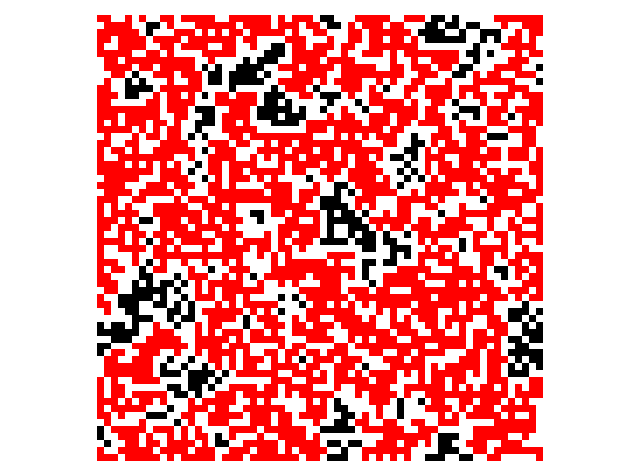
\includegraphics[height=80mm]{../plots/sample64}
		\caption{\label{fig:grid64} Sample lattice (L=64) where the spanning cluster is marked in red.}
\end{figure}

These probabilities satisfy the following equations:
\begin{align}
R_L^{(e)} &= 2R_L^{(h)}-R_L^{(b)}\\
R_L^{(1)} &= R_L^{(h)} -R_L^{(b)}
\end{align}
Therefore only two of them are independent. The reason we are interesting in the wrapping probabilities is that their values can be calculated exactly for an infinite lattice~\cite{Newman_2001}. The values to ten figures are given by:
\begin{align}
R^{(h)}_\infty(p_c) = 0.521058290\\
R^{(e)}_\infty(p_c) = 0.690473725\\
R^{(b)}_\infty(p_c) = 0.351642855\\
R^{(1)}_\infty(p_c) = 0.169415435
\end{align}
Now we can estimate $p_c$ as the solution $p$ of the following equation:
\begin{align}
R_L(p) =  R_\infty(p_c)
\end{align}
Our estimate of the mean of $R_L(p_c)$ over $n$ runs is drawn from the binomial distribution which has standard deviation:
\begin{align}
\sigma_{R_L} =\sqrt{\frac{R_L(p_c)[1-R_L(p_c)]}{n}}
\end{align}
We can evaluate the error by approximating $R_L(p_c)$ by the known value of $R_\infty(p_c)$. 
Ref.~\cite{Newman_2001} conjectures that $R_L(p_c)$ converges to $R_\infty(p_c)$ as $L^{-2}$. On the other hand, the width of the critical region decreases as $L^{-1/\nu}$, and therefore the gradient of $R_L(p)$ in the region goes as $L^{1/\nu}$. Thus the estimate of the critical occupation probability converges according to:
\begin{align}
p-p_c \sim L^{-2-1/\nu} = L^{-11/4}
\end{align}
Since for percolation on a square lattice we have $\nu = \frac 4 3$.

\subsection{Algorithm}

The Newman-Ziff algorithm was employed to simulate the system within the microcanonical ensemble.
The steps of the algorithm are as follows~\cite{Newman_2000}. The algorithm starts with an empty  lattice . As the lattice is populated in a random order, clusters are given a label identifying them. When a bond connecting two sites is added, they are either a member of the same cluster or they are members of two different clusters. In this second case, the labels need to be updated to reflect the fact that the bond has connected the clusters. 

In the interest of efficiency, the clusters are stored in an array mimicking a tree structure in which a site is chosen to be the "root" of the cluster. All other sites in the cluster point either to the cluster root or another site in the cluster. Starting from any site, the root node can be found by following these pointers. Clusters can be connected together by a adding a pointer from the root of one to the root of the other.

This type of algorithm is called \emph{weighted union–find with path compression}, weighted because the two trees are amalgamated by making the smaller a sub-tree of the other. Path compression signifies that the pointers of all traversed nodes are changed to point to the root node, in order to speed up the next searches. The steps taken to add one bond are roughly constant in time, therefore the algorithm adds N bonds in $\mathcal O(N)$ time.

In order find whether a configuration has percolated, additional work must be done. We add variables to each node which store the displacement to the parent node in both coordinates. Now the total displacement to the root node can be computed by traversing the tree and adding the displacements together. When a bond is added joining two sites $i$ and $j$ that are members of the same cluster, there are two paths from $i$ to the root node. One that goes through the parent of $i$ and another that consists of hopping to $j$ and then going through $j$'s parents. We sum the displacements along both of these paths, and percolation has occurred if the difference in displacement is equal to $\pm L$ in either of the coordinates~\cite{Mertens_2012}. 

The implementation of the algorithm was done in the C language, while Python libraries were used for the plots. The Mersenne Twister was the pseudo-random number generator employed. 

\section{Results from simulations}

\begin{figure}
	\centering
		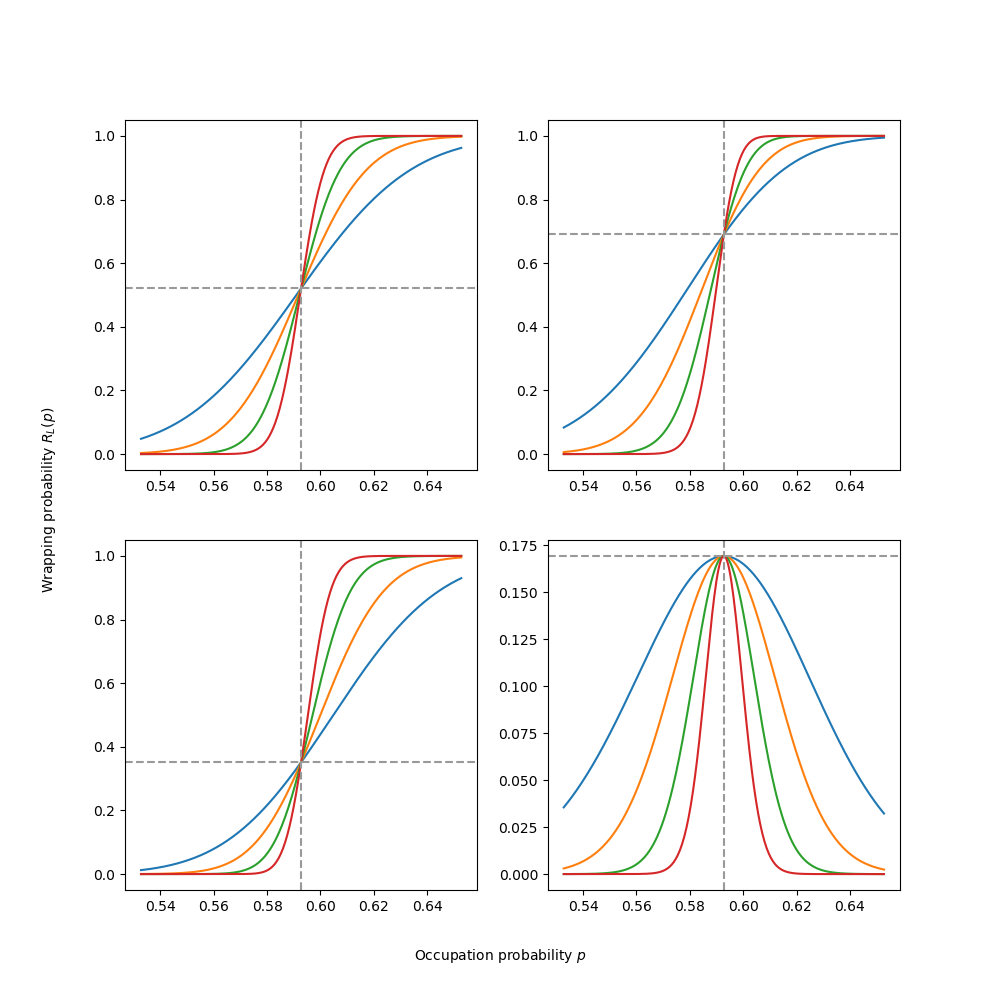
\includegraphics[width=\linewidth]{../plots/plot1}
		\caption{\label{fig:plot1} }
\end{figure}

\begin{figure}
	\centering
		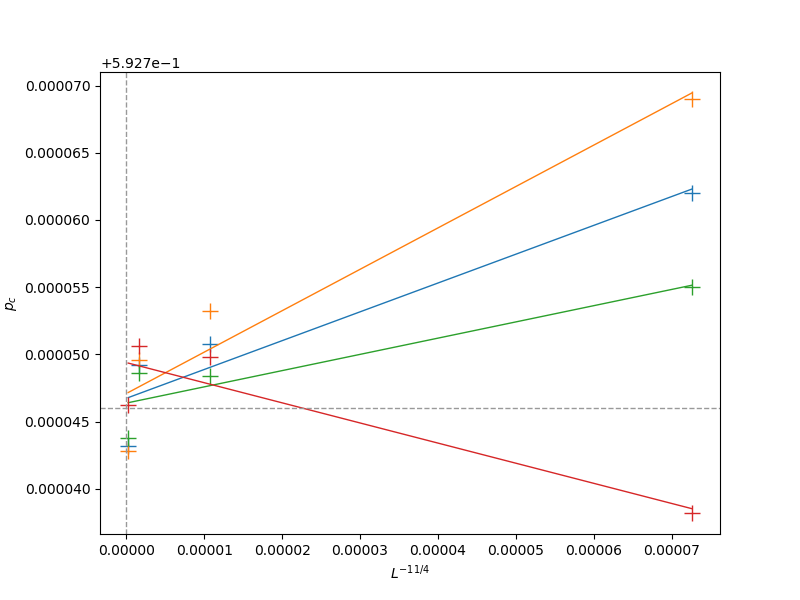
\includegraphics[width=\linewidth]{../plots/plot2}
		\caption{\label{fig:plot2} }
\end{figure}

\section{Conclusions and thoughts on further studies}
- more samples to get an accurate $p_c$, but the computation duration already was in the order of 10 hours
- without multi-threading and optimization, the computation would take weeks or months
- still an accurate value for the percolation threshold










